\documentclass[a4paper,11pt]{kth-mag}
\usepackage[T1]{fontenc}
\usepackage{textcomp}
\usepackage{lmodern}
\usepackage[utf8]{inputenc}
\usepackage[swedish,english]{babel}
\usepackage{modifications}
\usepackage{amsmath}
\usepackage{amsfonts}
\usepackage{listings}
\usepackage{alltt}
\usepackage{subfigure}
\usepackage{draftwatermark}
%\usepackage[firstpage]{draftwatermark}

\SetWatermarkLightness{0.9}
\SetWatermarkScale{1.1}

\usepackage{tikz}
\usetikzlibrary{automata,positioning,shapes.symbols}

\newcommand{\todo}[1]{\textbf{todo: #1}}
\newcommand{\rephrase}{\textbf{(rephrase)} }

\title{Test-inspired runtime verification}

\subtitle{Using a unit test-like
specification syntax for runtime verification}

\foreigntitle{"TODO: Test-inspirerad runtime-verifiering"}

\author{Adam Renberg}
\date{May 2012}
\blurb{Master's Thesis at CSC\\Supervisor Valtech: title? Erland
Ranvinge\\Supervisor CSC: title Narges Khakpour\\Examiner: title Johan Håstad}
\trita{TRITA xxx yyyy-nn}

\begin{document}

\lstset{basicstyle=\ttfamily, tabsize=2, showspaces=false,
showstringspaces=false, numbersep=20pt}

\frontmatter
\pagestyle{empty}
\removepagenumbers
\maketitle
\selectlanguage{english}




%================================================
%====== The Abstracts
%================================================

\begin{abstract}

Abstract in English. Write when most of the report is written.

\bigskip\noindent
Keywords: Runtime Verification, Unit Testing
\end{abstract}
\clearpage

\begin{foreignabstract}{swedish}

Sammanfattning på svenska. Skrivs sist.

\bigskip\noindent
Keywords (Sökord? Nyckelord?):
\end{foreignabstract}
\clearpage




%================================================
%====== The Preface and ToC
%================================================

\pagestyle{newchap}
\chapter*{Preface}

This is a master thesis / degree project in Computer Science at the Royal
Institute of Technology (KTH), Stocholm. The work was done at Valtech Sweden,
an IT Consultancy. It was supervised by Erland Ranvinge (Valtech) and Dr.
(\todo{check}) Narges Khakpour (CSC KTH).

\todo{Thanks to people}
\clearpage

\pagestyle{newchap}
\tableofcontents*
\mainmatter




%================================================
%====== Chapter 1, Introduction
%================================================

\pagestyle{newchap}
\chapter{Introduction} \label{chapter-introduction}

Due to the increasing size and complexity of computer software it has become
increasingly difficult, if not impossible, to convince oneself that the
software works as desired. This is where verification tools can be used to
great effect. Of these tools, testing is the one known by most and in wide
spread use.  The spread of agile development practices and test-driven
development has also popularized the concept of \textit{unit testing}, in which
small modules of a program or system are tested individually.

While testing is popular and often works well, it is incomplete and informal,
and thus yields no proof that the program does what it should - follow its
specification. Formal verification techniques, such as theorem proving, model
checking (and its bounded variant), can give such proofs, but they often suffer
from complexity problems (incompleteness, undecidability) and practical issues,
such as the so-called state explosion problem, and not being fully automated.

A relatively \rephrase new approach in this area is runtime verification, in
which the program \textit{execution} is verified against its specification.
With the specification written in a suitably formal language, the program can
be monitored to check that the specification is followed.


\section{Problem Statement} \label{section-problem-statement}

How can runtime verification specifications be written in a manner that uses
the syntax of the target program's programming language, and resembles
the structure of unit tests?

\section{Motivation}

Checking that a program works correctly is of great interest to software
developers, and formal verification techniques can often help. As mentioned
above, traditional approaches can be impractical with larger programs, and
verification by testing is informal and incomplete. Runtime verification can
here be a lightweight addition to the list \rephrase of verification
techniques.

The specification languages used by runtime verification approaches are often
based on formal languages/formalisms (e.g.\ logic or algebra) and not written in
the target program's programming language.  This means that writing the
specifications requires specific knowledge and expertise in mathematics.  It
also requires mental context-switching and special tools to support this
specialised language's syntax. In contrast, unit testing frameworks often
utilise the programming language to great effect, and their use is wide spread.

If runtime verification specifications more resembled unit tests, and were
written in the target program's programming language, it might popularise the
use of runtime verification for checking the correctness of software systems.

\section{Disposition}

Perhaps: Discuss the sectioning of this report.

The rest of this report is structured in as follows. Chapter 2 gives a
background to the subject of verifying program correctness. Chapter 3 continues
by describing the previous research on runtime verification and the syntax of
specification languages. It also gives an overview of the current ideas in unit
testing.

What will this report discuss? What problems? Why is this interesting?

What will this report \textbf{not} discuss?




%================================================
%====== Chapter 2, Background
%================================================

\pagestyle{newchap}
\chapter{Background} \label{chapter-background}

Runtime verification is a new area of research, but the research on
verification and formal methods goes back several decades. Research of interest
include the early work on formal methods, e.g.\ by Hoare \cite{hoare69} and
Floyd \cite{floyd67}, and work on logics suitable for runtime verification,
e.g. LTL by Pnueli \cite{pnueli77}. The seminal work done by Hoare, Floyd and
Pnueli lay the foundation for many interesting approaches used for runtime
verification. LTL is one of the common formal languages used for formal
specifications in runtime verification.

This chapter gives a short overview of the background to the concepts of this
report. It starts with laying out what we mean by proving the correctness of
programs in Section~\ref{section-proving-correctness}. Section~\ref{section-rv}
describes runtime verification and its place in proving correctness. And
finally, Section~\ref{section-testing} discusses testing.


\section{Proving Correctness} \label{section-proving-correctness}

A correctness proof is a certificate, based in mathematics and logics, that a
program/system/function follows its specifications, i.e.\ does what it is
supposed to do. There are several approaches, with their advantages and
disadvantages.

\textit{Theorem proving}, as started by Hoare \cite{hoare69}, Floyd
\cite{floyd67} and others, is the manual, semi-automated, or (not so often)
fully automated process of mathematically proving that the system follows its
specification. There are many ways of doing such proofs.

One way is to prove that at all points in the program, given inputs satisfying
some pre-conditions, the outputs will satisfy the post-conditions. By
formulating the post-conditions of the exit point(s) so that they follow the
specification, and by linking together the pre-conditions of program points
with their preceding program points' post-conditions, we now know that correct
indata will yield correct results.

This way of proving correctness often yields the best results. But it is slow,
hard to automate, and therefore requires much manual labor. Wading through
large programs thus often becomes impractical.

\textit{Model checking} is the concept of verifying that a \textit{model} of a
system follows its specification. This requires that both the model and the
specification is written in a mathematical formalism. Given this, the task
becomes to see if the model satisfies a logical formula. It is often simpler
than theorem proving, and can be automated.

The model of the system is usually structured as a finite state machine, and
verification means visiting all accessible states, checking that they follow
the specification. This can be problematic, especially when the state space
becomes very big, something known as the \textit{state explosion problem}.
There are approaches to address this issue, such as \textit{bounded model
checking}, or by using higher-level abstractions.

Proving that a model of a system is correct can be very useful, but it suffers
from the inherent flaw of only verifying the model, not the actual system. The
model can be difficult to construct, or deviate too far from the system.
Runtime verification attempts to solve this by dealing directly with the
system, creating its model during runtime.


\section{Runtime Verification} \label{section-rv}

Much in common with model checking. Only current execution. Finite traces.
Dynamic environment.

Runtime verification (RV) is a dynamic approach to checking program
correctness, in contrast to the more traditional formal static analysis
techniques discussed above. These are often very useful, but suffer from severe
problems such as the state explosion problem, incompleteness, undecidability
etc., when they are used for verification of large-scale systems.  Moreover,
static analysis usually verifies an abstract model of the program, and cannot
guarantee the correctness of the implementation or the dynamic properties of
the executing code.

Runtime verification aspires to be a light-weight formal verification
technique, see e.g.\ \cite{leucker09abriefaccount,delgado04taxonomy}. It
verifies whether some specified properties hold during the execution of a
program.

The specification that should be verified is often written in a formal
language, often a logic/calculus, such as linear temporal logic
\cite{pnueli77}. To build a \emph{system model} for verifying the properties of
the specification, the target program needs to emit and expose certain events
and data. The collected events and data are used to build the system model.
Many RV frameworks use \textit{code instrumentation} to generate
\textit{monitors} for this end.

There are two types of monitoring: \emph{online} and \emph{offline}. In online
monitoring, the analysis and verification is done during the execution, in a
synchronous manner with the observed system. In offline monitoring, a log of
events is analysed at a later time.

When a violation of the specification occurs, simple actions can be taken
(e.g.\ log the error, send emails, etc.), or more complex responses initiated,
resulting in a \textit{self-healing} or \textit{self-adapting} system (see
e.g.\ \cite{huebscher08survey}).

Relevant work on runtime verification include \cite{bauer06monitoring}, in
which Bauer et al.\ use a three-valued boolean logic (true, false and ?) to
reflect that a specification can not only be satisfied (true) or violated
(false), but also neither yet, or, in the future it may be either. Bauer et
al.\ also show how they transform specifications into automata (i.e.\ runtime
monitors). Bodden presents in \cite{bodden05efficientrv} a framework for RV
implemented through \emph{aspect-oriented programming} \cite{aspectj} in Java,
with specifications written as code annotations.

Leucker et al.\ present a definition of RV in \cite{leucker09abriefaccount},
together with an exposition on the advantages and disadvantages, similarities
and differences, with other verification approaches. In
\cite{delgado04taxonomy}, Delgado et al.\ classify and review several different
approaches and frameworks to runtime verification.


\section{Testing} \label{section-testing}
On the other end of the program-correctness-checking spectrum is
\emph{testing}, which is the practical approach of checking that the program,
given a certain input, produces the correct output.  Testing is not complete,
and lacks a formal foundation, so it cannot be used for formal verification.
Testing can be a complement to more formal techniques, such as RV (but is in
many cases the sole correctness-checking tool).

Unit testing is quite young, perhaps having begun in earnest in the 90s, and it
was popularized by the extreme programming (XP) movement \todo{cite someone}.
Testing in general is very old.

Kent Beck introduced the style of the modern unit testing framework in his work
on a testing framework  for Smalltalk \cite{becksmalltalktesting}.  Together
with Eric Gamma he later ported it to Java, resulting in JUnit \cite{junit}.
Today, this has lead to frameworks in several programming languages, and they
are collectively called xUnit \cite{fowlerxunit}.

\textit{Unit testing} is the concept of writing small tests, or test suites,
for the units in a program, such as functions, classes, etc. These tests are
used during development to test the functionality of the units. They aim to
reduce the risk of breaking existing functionality when developing new features
or modifying existing code (by preventing regression).

Writing unit tests, often using unit testing \textit{frameworks} such as JUnit
\cite{junit} for Java and unittest \cite{python-unittest} for Python, is a
common practice on many development teams.

Testing is not formal - it doesn't prove anything except that the program works
for the provided test cases. Testing is also not complete - for all but the
most trivial programs, it is impossible to write tests for all cases.

Testing is often a manual process, taking up a large part of development time
(see e.g.\ \cite{brooks75mythicalmanmonth}). Still, there are tools to automatically
generate tests.

When discussing testing, and unit testing in particular, we must mention the
concept of test-driven development (TDD). Also made popular by XP, it consists
of the cycle: (1) write a failing test, (2) make it pass by writing the
simplest code you can, and (3) refactor, rewrite the code so that it is good.
Tests here play the part of specifications for the units of the program.

\todo{Find correct places to cite. Original book on TDD?}




%================================================
%====== Chapter 3, Previous Research
%================================================

\pagestyle{newchap}
\chapter{Previous Research} \label{chapter-previous-research}

As we saw in Section~\ref{section-rv}, runtime verification is the technique of
verifying a program's compliance against a specification during runtime. These
specifications need to be written somehow, which will be discussed in
Section~\ref{section-specifications}. Approaches for verification are discussed
in Section~\ref{section-verification}. For verification to work, during
runtime,
the program usually needs to be instrumented in such a way that the
verification process can access all pertinent data. This is discussed in
Section~\ref{section-instrumentation}

The design of unit test syntax is discussed in
Section~\ref{section-unit-testing}. The combination of the two, runtime
verification and unit testing, will be the main subject in
Chapters~\ref{chapter-method} and~\ref{chapter-results}.


\section{Specifications} \label{section-specifications}

Specifications come in many forms, from the informal ones like "I want it to be
easy to use", to the contractual ones written by companies and clients, to the
ones written in formal languages, specifying properties that should verifiably
hold about the program. It is this last type of specifications we are
interested in here, and which play an important role in runtime verification.

In general, specifications should be abstract, written in a high-level
language, and succinctly capture the desired property. Writing erroneous
specifications is still possible; specifications need to be easier for humans
to verify than the program's implementation. There is little point to have a
specification as complex as the program itself, except as a point of reference.
A program can, of course, be seen as a all-encompassing, perfect, always-true,
specification of itself.


\subsection{Formalisms for Specifications}

There are several common formalisms for writing specifications, and many papers
that expand, rephrase and illuminate on them. Although they can be quite
different, they share a common origin in the work done by Floyd \cite{floyd67},
Hoare \cite{hoare69}, and others before them.  Floyd thought of formulas
specifying in/out properties of statements, and chaining these together to form
a formal proof for the program. Hoare elaborated on this idea by basing his
proofs on a few axioms of the programming language and target computer
architecture, and building the proof from there.

\subsubsection{Linear Temporal Logic}

Linear Temporal Logic (LTL) was first discussed by Pnueli in \cite{pnueli77},
and has since been popular in many areas dealing with a system model containing
a temporal dimension. As Pnueli describes it, it is simpler than other logics,
but expressive enough to describe many problems of interest for verification.
This has been "confirmed" \rephrase by the diverse use of LTL by many
researchers \todo{citations}.

LTL uses a system model of infinite execution traces, or histories, of the
states of the execution. LTL specifications are formulas that operate on these
states. An LTL formula consists of \textit{propositional variables} that work
on the domain model of the state (checking variables, global state, etc.), the
normal logical operators such as negation and disjunction, and some temporal
operators. The most basic and common temporal operators are $\boldsymbol{X}$,
\textit{next}, and $\boldsymbol{U}$, \textit{until}. Other operators can be
derived from these, such as $\boldsymbol{G}$, \textit{globally}, and
$\boldsymbol{F}$, \textit{eventually}.

Bauer et al.\ introduce a three-valued boolean logic LTL$_3$ in
\cite{bauer06monitoring}, taking the values (true, false and ?). This logic is
arguably more suited for the finite nature of runtime verification, whereas LTL
was designed with infinite traces in mind. The semantics of LTL$_3$ reflect the
fact that when verifying runtime verification specifications, can not only
be satisfied or violated, but inconclusive. For satisfied or violated
specifications, no further verification is required - we already know the
outcome. For inconclusive verification, we need to continue verification, as,
with future events, the result could be either or.

An example LTL formula, taken from a list of common specification patterns
\cite{dwyer99patterns}, could be: $S$ precedes $P$, i.e.\, if the state $P$ holds
sometime, the state $S$ will hold before it. This is shown in
Figure~\ref{figure-ltl}.

\begin{figure}[h!]

\[
\boldsymbol{G} \, P \rightarrow (\neg P \, \boldsymbol{U} \, (S \wedge \neg P)
\]

\caption{An example of an LTL formula. This can be read as: Globally, if $P$
holds, then, while $P$ didn't hold, $S$ held at some point.}
\label{figure-ltl}
\end{figure}

There is a counterpart to LTL in the real-time setting called Timed Linear
Temporal Logic \todo{cite someone}. It introduces clocks to make specifications
of real-time properties possible. It is of great interest to runtime
verification, but won't be discussed further here. \todo{See [] and [] for more
on TLTL}.

\subsubsection{EAGLE?}

What about EAGLE?

\subsubsection{CPL}

Hmm, CPL?


\subsubsection{Design by Contract}

Design by Contract was introduced by Bertrand Meyer in \todo{where}, and has
been fully implemented in the Eiffel programming language. A contract is the
idea that functions, and methods on objects, promise to fulfill certain
post-conditions (or promises) if the inputs they are given fulfill the
pre-conditions (or requirements) in the contract. Design by Contract also
contains constructs for specifying loop-invariants and class-invariants,
properties that should always hold during loops and for objects of a class,
respectively. Assertions (see below) are also usually available.

Design by Contract is inspired by Hoare logic, and is essentially Hoare logic
written in a certain style.


\subsubsection{Assertions}

A common construct that is part of many popular programming languges, like C,
Java, Python, is the assertion statement. It is a way to assert that some
predicate holds at a point in the program. Usually the predicate is an
expression of the programming language, and is not supposed to alter the
program state.

Assertions are distinct from the normal program flow, and not to be confused
\rephrase with exceptions. Assertions check for properties that should always
be true, anything else would be a programming error.


\subsection{Writing Specifications}

For verification in general, specifications can be written and used externally
to the program. They can be used in specialized model-checking tools, in tools
for theorem proving etc.

Runtime verification requires that the specifications are accessible when
building and running the program. At the very least, the program needs to be
instrumented \rephrase to expose the correct system model so that the
specification can be verified. It is often \rephrase desired in runtime
verification to do online verification, and then the specifications need to be
available and embedded into the system. A few approaches have been taken to
enable this.

Approaches to writing specifications can be divided into two parts: those that
require you to manually mark code for verification, and those that inject the
verification code from external specifications.

Rosuenblum \cite{rosenblum95practicalassertions} uses specially annotated
comments. Bodden \cite{bodden05efficientrv} uses Java annotations, which are
written at function and variable definitions, to mark code for verification.
\todo{more, and rephrase}. The programming language Eiffel has full language
support for Design by Contract, with pre- and post-conditions, invariants, and
more. Other approaches \todo{who?} use external specification files. For simple
cases it is common to write assertions in the program, checking boolean
expressions under runtime \todo{cite jass}.


\section{Verification against Specifications} \label{section-verification}

Formal specifications are written so that programs can be verified against them
- to see whether they follow the specification, or violate parts of it.

There are several ways to verify a program against its specification. A common
one, used in \cite{bauer06monitoring,bodden05efficientrv} among others, is to
generate state machines from the specification. These state machines, often
called \textit{monitors}, operate with the input language of events emitted by
the program.

\todo{Monitors. Büchi Automatons.}


\section{Code Instrumentation} \label{section-instrumentation}

For verification to work, the verifier (such as a monitor) needs access to
events happening in the program. Such events can be functions called,
statements executed, variables assigned, etc., depending on the system model of
the specification language \rephrase. The program needs to be instrumented for
it to emit such events. This often means wrapping function calls and variable
assignments in a "recording layer", which performs the desired action after
logging the event. The events can then be "sent" to the verification tools.


\subsection{Pre-processing the Code}

Rosuenblum \cite{rosenblum95practicalassertions} uses a pre-processor step in
the C compilation setup instrument code, where the specifications (called
assertions there) are written adjacent to the code under watch.


\subsection{Post-processing the Code}

It is also possible to rewrite the compiled program, instrumenting the code
after compilation. This way, the program needs no knowledge of the verification
framework.


\subsection{Dynamic Code Rewriting}

In many dynamic languages, such as Python, Ruby or Javascript, it is possible
to rewrite the code during runtime, which is sometimes called monkey patching.
A function to be monitored could be rewritten, adding a lightweight wrapper
that records all calls to it, and then delegates to it.


\subsection{Aspects}

An interesting approach to external injection is to use aspect-oriented
programming. In aspect-oriented theory, a program is divided into modules, each
only dealing with their own \textit{concern}. Logging, for instance, is a
\textit{crosscutting concern}, as it is used by all modules. The goal is to not
scatter all logging code across all modules, and to not tangle it with the
modules' logic. This can be done by defining the logging code as
\textit{aspects}, which consists of the logging code, called the
\textit{advice}, and the \textit{point cut}, which is a formula describing when
the advice should be executed. The possible execution points \rephrase for a
point cut are called \textit{join points}.

Runtime verification is a typical case of a cross-cutting concern. Bodden
\cite{bodden05efficientrv} uses it in his runtime verification implementation.

Aspects are often implemented as a post-processing step in the compilation
process, adding code for handling the aspects.


\section{Unit Testing} \label{section-unit-testing}

We discussed testing and unit testing in general in
Section~\ref{section-testing}. How does unit testing work? What is the
syntaxes? This section mostly concerns the language and syntax used for writing
unit tests.

\subsection{xUnit}

The xUnit style of unit testing \cite{fowlerxunit} has given rise to unit
testing frameworks for many programming languages. Their structure are all
based on the same concept, and since JUnit is the canonical, and one of the
first, implementation, I'll use it for a short demonstration. See
Figure~\ref{figure-junit}.

\begin{figure}[h!]
\lstset{language=Java}
\begin{lstlisting}
// required imports removed for brevity

public class TestSomeClass extends TestCase {
	private Environment;

	@Before
	public void setUp() {
		// setup the fixture for each test
		Environment = new Environment();
	}

	@After
	public void tearDown() {
		// clean up the fixture, free memory, etc.
	}

	@Test
	public void testSimpleAddition() {
		// use the language assertion construct
		assert 1+1 == 2
		// use JUnit's assertion functions
		assertEquals(4+7, 11)
	}

	@Test
	public void testThatDoWorkReturnsX() {
		// do setup for this test
		Target t = new Target(...);
		// exercise the object under test
		t.doWork(...);
		// do verification
		assert t.getValues() == x;
	}
}
\end{lstlisting}
\caption{An example of unit testing syntax, written as a test case for JUnit.}
\label{figure-junit}
\end{figure}

In JUnit, and xUnit, you run a \textit{test suite} of \textit{test cases},
which contain tests. The example in Figure~\ref{figure-junit}, the test suite
is implicitly created by JUnit, although it is possible to create it and
control it your self. A \textit{test runner} runs the test suite, showing
progress to the user.  When the tests are finished, any errors are shown to the
user.

The example in Figure~\ref{figure-junit} has two tests, and methods to set up
and tear down the tests \textit{fixture}. The fixture is the surrounding set of
objects (environment) that the object under test requires to work properly.
These functions are usually called \textit{setUp} and \textit{tearDown},
respectively.

The order in which tests are executed is arbitrary in JUnit. One possible
ordering of the relevant methods in the example is:

\begin{enumerate}
	\item \textit{setUp}
	\item \textit{testSimpleAddition}
	\item \textit{tearDown}

	\item \textit{setUp}
	\item \textit{testThatDoWorkReturnsX}
	\item \textit{tearDown}
\end{enumerate}

Test written in this style are traditional unit tests. 

\todo{Mocking? This is "TDD"-style}

\subsection{Behaviour-driven Development}

There is a style of writing tests called behaviour-driven development
\cite{north06bdd}. It originated from test-driven development, and is built on
the idea that the tests you write should test the behaviour of the program. The
simplest example is that you write your unit tests after the behaviour you
desire, perhaps naming your tests according to "X should do Y". A more radical
example is shown in Figure~\ref{figure-bdd}.

\begin{figure}[h!]

\begin{alltt}
+Scenario 1: Account is in credit+
\textit{Given} the account is in credit
\textit{And} the card is valid
\textit{And} the dispenser contains cash
\textit{When} the customer requests cash
\textit{Then} ensure the account is debited
\textit{And} ensure cash is dispensed
\textit{And} ensure the card is returned
\end{alltt}

\caption{An example scenario describing a behaviour, as written in BDD.
Scenario taken from \cite{north06bdd}.}
\label{figure-bdd}
\end{figure}

The test runner parses each scenario, and for each line finds a matching unit
of code that does what the line describes. This way of writing tests, or
describing behaviours, leads to a outside-in, or top-down, way of writing and
thinking about your program.

\subsection{Mocking and Faking}

A common issue when writing unit tests is that, to instantiate some object X,
or to call some function Y, the program needs access to some other
objects/data/configuration Z. Z might be something simple, which we can easily
create in the test. It might also be a network or database connection, or
something doing heavy calculation, or just something complex.

One way to work around this is to create fake/mock/dummy, objects. A fake
network connection has the same interface as a real network connection, but
calling it doesn't actually transmit anything anywhere, and it might return
hard coded data. Fake objects could save what actions are taken upon them, and
the test could then verify that these are according to expectations.

\subsection{Expectations}

Instead of writing fake objects, we can create a mock object and pre-record
what actions we expect to be taken upon them. This is called writing
\textit{expectations} \cite{fowler07expectations}. A simple example of
expectations is shown in Figure~\ref{figure-expectations}.

\begin{figure}[h!]

\lstset{language=Java}
\begin{lstlisting}
public class OrderInteractionTester extends MockObjectTestCase {
	private static String TALISKER = "Talisker";

	public void testFillingRemovesInventoryIfInStock() {
		// setup - data
		Order order = new Order(TALISKER, 50);
		Mock warehouseMock = new Mock(Warehouse.class);

		// setup - expectations
		warehouseMock.expects(once()).method("hasInventory")
			.with(eq(TALISKER),eq(50))
			.will(returnValue(true));
		warehouseMock.expects(once()).method("remove")
			.with(eq(TALISKER), eq(50))
			.after("hasInventory");

		// exercise
		order.fill((Warehouse) warehouseMock.proxy());

		// verify
		warehouseMock.verify();
		assertTrue(order.isFilled());
	}
}
\end{lstlisting}

\caption{An example of expectations, written using jMock and JUnit.
Example taken from \cite{fowler07expectations}.}
\label{figure-expectations}
\end{figure}

Figure~\ref{figure-expectations} shows a test of a fictional shop. The test
tests only one thing, the fill method of the Order object, but it requires a
Warehouse object, for access to the inventory. We supply a mock Warehouse, with
expectations on which methods should be called on it, with which arguments and
what they should return.

An expectation follows a simple pattern:

\begin{itemize}
	\item Object (optional) and function.
	\item Invocation count, how often is the function expected to be called
	\item Expected arguments. Can be explicit values, or generic types, or
		ignored.
	\item What should happen, e.g.\ what the function should return.
	\item When this should happen, e.g.\ in what sequence of function calls, in
		what global state.
\end{itemize}

There are two common ways of specifying expectations: recording and explicit
specification. Figure~\ref{figure-expectations} shows an example of how to
explicitly specify expectations.

When recording expectations, you create a mock object and call the expected
functions, with expected arguments and return values, in the expected order.
Then you set the mock into replay mode, and it will replay the recorded
expectations, and verify that they occur correctly.

There are several frameworks for working with expectations, such as
jMock\footnote{\texttt{http://www.jmock.org/}} for Java, Rhino
Mocks\footnote{\texttt{http://ayende.com/wiki/Rhino+Mocks.ashx}} and
Ludibrio\footnote{\texttt{https://github.com/nsigustavo/ludibrio/}} for Python.





%================================================
%====== Chapter 4, Method
%================================================

\pagestyle{newchap}
\chapter{Method} \label{chapter-method}

As stated in Section~\ref{section-problem-statement}, the objective of this
thesis is to investigate whether it is possible to do runtime verification with
specifications written in the target program's programming language, structured
similar to unit tests. To find a solution to this, there are four issues we
need to address:

\begin{enumerate}
	\item How should the syntax for the specification be defined, so that it
		looks similar to that for unit tests, but works for runtime verification?
		Which language could be used? Which unit testing framework to take
		inspiration from?
	\item How should the program be instrumented to monitor the system, to expose
		the appropriate events and data, and to build the system model?
	\item How will this be used to verify the system against the
		specification? Online or offline verification? E.g.\ which techniques
		should be used to verify the monitored system against the specification?
	\item How can it be provided with a formal foundation?
\end{enumerate}

This report is a documentation on how to solve these issues. The following
sections are each dedicated to one issue, and shows a proof-of-concept of these
ideas. The implementation, called \textit{pythonrv}, can be found
online\footnote{\texttt{https://github.com/tgwizard/pythonrv}}.

\section{Definitions}

Define some stuff first? Instrumentation? "The function to be monitored"?
Specification function? Specification?

\section{Syntax}

During the development of this proof-of-concept, the biggest factor in deciding
what language to use was how it would assist in instrumentation.
Instrumentation is discussed in Section~\ref{section-method-instrumentation}.
Python was chosen as the implementation language.

The canonical framework for doing unit testing in Python is the unittest2
framework that is included in all modern versions. Not much development has
happened on it in the last years. Many new frameworks have have spawned, such
as PyUnit, Nose and py.test. They build upon the style of unittest2, and mostly
add new miscellaneous features, and better test reporting. The original
structure of the unit tests is still prevalent. unittest2 builds on the xUnit
style, discussed in Section~\ref{section-unit-testing}.

A few simple example below will introduce the syntax of pythonrv. After that
the capabilities and limitations of the current implementation will be
exposited.

\subsection{Three Examples}
\lstset{language=Python,numbers=left}

\begin{figure}[h!]

	\begin{center}
	\begin{minipage}{0.7\textwidth}
	\lstinputlisting{figures/syntax_example_1.py}
	\end{minipage}
	\end{center}

	\caption{A specification that monitors the function \texttt{fib} in the
		module \texttt{fibmodule}. The monitored function is, locally to the
		specification, aliased as \texttt{func}. The specification asserts that the
		first input to the monitored function is always greater than zero.}
	\label{figure-syntax-example-1}
\end{figure}

The example in Figure~\ref{figure-syntax-example-1} shows the basics of a
pythonrv specification. Line 1 imports the rv module from the pythonrv package.
On line 2 it imports the module(s) containing the function(s) we wish to
monitor. Line 5 defines the specification as an ordinary python function called
\texttt{spec}, taking one argument, \texttt{event}. The instrumentation is done
line 4 by using the \textit{function decorator}\footnote{See
Section~\ref{section-method-instrumentation} for an explanation.}
\texttt{rv.monitor}. \texttt{rv.monitor} declares that the function
\texttt{fib} in \texttt{fibmodule} should be monitored, and, whenever
\texttt{fib} is called, \texttt{spec} should be called as well.


The specification itself consists of any valid python code. It has access to a
special argument, \texttt{event}, which gives the specification function access
to data about the current event. On line 6, the array of input arguments used
to call \texttt{fib} is accessed to check that the first argument is greater
than zero.

The specification function in Figure~\ref{figure-syntax-example-1} will be
called upon every invocation to \texttt{fibmodule.fib}.

\begin{figure}[h!]

	\begin{center}
	\begin{minipage}{0.7\textwidth}
	\lstinputlisting{figures/syntax_example_2.py}
	\end{minipage}
	\end{center}

	\caption{A specification that monitors two functions, \texttt{mymodule.foo}
	and \texttt{mymodule.bar}. It asserts that calls to the two functions
alternate; that no two calls to \texttt{foo} occurs without a call to
\texttt{bar} in between, and vice versa. The first call has to be to
\texttt{foo}.}
	\label{figure-syntax-example-2}
\end{figure}

Figure~\ref{figure-syntax-example-2} shows how a specification can monitor two
functions. The specification function will be called whenever either of the
monitored functions is called. Which function was called can be determined from
the \texttt{event} argument, as is done on lines 6 and 9. It is the
\texttt{called} attribute of a function in the \texttt{event.fn} structure
allows for this.

The example also shows how the specification can access a history of previous
events - events that it has handled in the past. \texttt{event.history} is a
list of all events that has occurred - that this specification monitors. The
last element is the current event, and the next-to-last element is the previous
element, which can also be accessed as \texttt{event.prev}.

\begin{figure}[h!]

	\begin{center}
	\begin{minipage}{0.7\textwidth}
	\lstinputlisting{figures/syntax_example_3.py}
	\end{minipage}
	\end{center}

	\caption{A more complex example: A specification function that monitors three
		functions, \texttt{foo}, \texttt{bar} and \texttt{baz}, and makes sure that
		\texttt{foo} is called first, then any number calls to \texttt{bar} with
		the first argument as \texttt{True}, and then finally a call to
	\texttt{bar}. After that, any calls are allowed - the specification function
won't be verified any longer.}
	\label{figure-syntax-example-3}
\end{figure}

Figure~\ref{figure-syntax-example-3} shows a more advanced example, in which
the \texttt{next} function of the \texttt{event} argument is used.
\texttt{next} allows the specification function to add more specification
functions (possibly implemented as closures or lambdas) to be executed when the
next event occurs.

On line 9 the function \texttt{followup} is added to be executed on the next
event. Since \texttt{followup} is added in this way - as a "oneshot"
specification - it needs to add it self using \texttt{next} for verification on
multiple events. This is done on line 22.

Figure~\ref{figure-syntax-example-3} also shows how a specification function
can turn its verification off - unsubscribe from future events.
\texttt{event.finish} and \texttt{event.success} are essentially the same, and
unsubscribes without further errors. \texttt{event.failure} can be thought of
as a combination of \texttt{event.finish} and \texttt{assert False} (which
always fails).


\subsection{Capabilities and Limitations}

\todo{}

Write about the details of the \texttt{rv.monitor} and \texttt{rv.spec}
function decorators, and about the uses of the \texttt{event} argument. Also
shortly describe how one can configure custom error handlers to take action
when verification fails (or do this in the verification section).

\section{Instrumentation} \label{section-method-instrumentation}

The three examples in the previous section showed how pythonrv specification
functions can be written. This section will describe how these functions can
jack themselves into the ordinary control flow of the program and gain access
to the function call events and their arguments.

The instrumentation is performed through the \texttt{rv.monitor}
\textit{function decorator} in pythonrv. A python function decorator is similar
to attributes in .Net and annotations in Java. It is essentially a function
that takes a function, possibly modifies it, or uses it in some way (decorates
it), and then returns it - or some other function. This is used throughout
python to make static and class methods, for instance.
Figure~\ref{figure-function-decorator} shows an example function decorator
definition, and Figure~\ref{figure-function-decorator-usages} shows how to use
it.

\begin{figure}[h!]

	\begin{center}
	\begin{minipage}{0.7\textwidth}
	\lstinputlisting{figures/function_decorator.py}
	\end{minipage}
	\end{center}

	\caption{An example of how to define a function decorator.}
	\label{figure-function-decorator}
\end{figure}

\begin{figure}[h!]

	\begin{center}
	\begin{minipage}{0.7\textwidth}
	\lstinputlisting{figures/function_decorator_usages.py}
	\end{minipage}
	\end{center}

	\caption{An example of how to use the function decorator in
	Figure~\ref{figure-function-decorator}.}
	\label{figure-function-decorator-usages}
\end{figure}

\texttt{rv.monitor} first takes arguments specifying what functions should be
monitored, and then the specification function itself.

In python, almost all\footnotemark\ functions belong to a container of some
sorts - a class, an object, or a module. In
Figure~\ref{figure-function-decorator-usages} the functions \texttt{func\_a}
and \texttt{func\_b} belong to the module \texttt{test} (the module's name is
the same as that of the file containing the code). These containers are
essentially dictionaries (\textit{dicts} in python parlance) of key-value
pairs, where the keys in this case are function names and the values are
objects representing the function code. (There are other types of values in
these containers as well, which we can ignore).

\footnotetext[3]{This is not true of closures - function defined inside other
functions. These functions cannot be directly referenced outside the defining
function. pythonrv does not (as of writing) support monitoring of closures.}

The instrumentation in pythonrv works as follows. First, a wrapper function is
defined for each function to be monitored. This wrapper function's main purpose
is to call the specifications attached to the monitored function, and then call
the monitored function itself. The wrapper also does some argument copying and
such, to prevent side-effects in the specifications from interfering with the
monitored function. The container of the monitored function is then extracted,
and the reference to the monitored function is overwritten with a reference to
the wrapper. See Figure~\ref{instrumentation-overview} for a pseudo-python
overview.

The implementation of the instrumentation code in pythonrv is more optimized
than this - for instance, only ever one wrapper per monitoree is created,
independent of the number of specifications that want to monitor it.

\begin{figure}[h!]

	\begin{center}
	\begin{minipage}{0.7\textwidth}
	\begin{lstlisting}
# rv.py
def monitor(monitorees, specification):
	for monitoree in monitorees:
		# define a wrapper for each monitoree
		def wrapper(*args, **kwargs)
			event = create_event(...)

			# call specification
			specification(event)

			# call the actual function - the
			# monitoree
			return monitoree(*args, **kwargs)

		# overwrite the monitoree in its container
		container = get_container(monitoree)
		setattr(container, monitoree.name, wrapper)
	\end{lstlisting}
	\end{minipage}
	\end{center}

	\caption{An overview of the pythonrv instrumentation process, in
	pseudo-python. This is just for illustrative purposes and not how pythonrv
actually does the instrumentation.}
	\label{figure-instrumentation-overview}
\end{figure}


\section{Verification}

Veriaofsdjfaoisdjfaoisdfjalöskdfjalksfhaklsjdhflaksjhdf löadjsf ölaksdhf
öajksdhf lkasdhf kashdf öashf lkajshf ölaksdhf öaklsdf aölksdf öalksdjf aölsdjf
aölsdjf alöksdfj aölsdkfj 


\section{Formal Foundation} \label{section-method-syntax}

This is the most difficult part, and I really figured it out yet. What follows
is an early attempt at it.

A seemingly insurmountable problem quickly arises when attempting to give a
formal foundation to the specifications described in
Section~\ref{section-method-syntax}. The specifications are written as ordinary
python functions and, as such, are difficult to formalize. Python as a language
is rather informal - one implementation of it, CPython, serves as the reference
implementation.

One way to go around this is to define a semantics for a subset of python.
Specifications written in this subset will have a formal semantics, and they
will have a way to formally prove their correctness.

One formal semantics that can quite easily be ascribed to python code is that
of finite automata. The python code is translated into a finite automata. To
make this more manageable, translations are shown for some small "types of
python specifications", which can be composed to yield more complex
specifications. Proofs can thus use structural induction to prove general
properties no specifications.

The system model for the automata, the alphabet it works on, is the events of
the function(s) that a specification monitors. \todo{Currently the
specifications below only allow for one monitored function per specification.}

The idea with the transitions in the automata is that either we always follow a
transition, and we label it $\Sigma$, or we follow a transition only if the
event that has occurred satisfies some predicate $P$. If no transition fits,
the specification has been violated.

One peculiarity should be noted: On each new event, a new "instance" of the
automaton is spawned, starting from the beginning. All current "executions" of
the automaton is also continued.

Next follows the four specification modules I think are required. Their
presentation is quite ugly, unfortunately.

%%%%
%% null spec
\begin{figure}[h!]

	\begin{minipage}{0.45\textwidth}
		\centering
		\lstset{language=Python}
		\begin{lstlisting}
		def null_spec():
			pass
		\end{lstlisting}
		\subcaption{The \textit{null specification}, in python function format.}
	\end{minipage}
	~
	\begin{minipage}{0.45\textwidth}
		\centering
		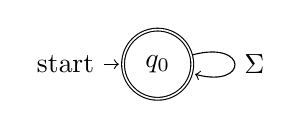
\begin{tikzpicture}[shorten >=1pt,node distance=2cm,on grid,auto,scale=.5]
			\node[state,initial,accepting] (q0)   {$q_0$};
			\path[->]
				(q0) edge [loop right] node {$\Sigma$} (q0);
		\end{tikzpicture}
		\subcaption{The \textit{null specification}, as an automaton.}
	\end{minipage}

	\caption{The \textit{null specification} - the simplest of specifications.}
	\label{label-spec-null}
\end{figure}

%%%%
%% assert spec
\begin{figure}[h!]

	\begin{minipage}{0.45\textwidth}
		\centering
		\lstset{language=Python}
		\begin{lstlisting}
		def assert_spec():
			assert P
		\end{lstlisting}
		\subcaption{The \textit{assert specification}, in python function format.}
	\end{minipage}
	~
	\begin{minipage}{0.45\textwidth}
		\centering
		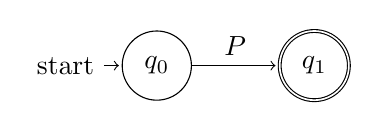
\begin{tikzpicture}[shorten >=1pt,node distance=2cm,on grid,auto,scale=.5]
			\node[state,initial] (q0)									{$q_0$};
			\node[state,accepting] (q1) [right of=q0]	{$q_1$};
			\path[->]
				(q0) edge node {$P$} (q1);
		\end{tikzpicture}
		\subcaption{The \textit{assert specification}, as an automaton.}
	\end{minipage}

	\caption{The \textit{assert specification} - the simplest specification that
	actually does something.}
	\label{label-spec-assert}
\end{figure}

%%%%
%% next spec
\begin{figure}[h!]

	\begin{minipage}{0.45\textwidth}
		\centering
		\lstset{language=Python}
		\begin{lstlisting}
		def next_spec():
			next(any_spec)

		\end{lstlisting}
		\subcaption{The \textit{next specification}, in python function format.}
	\end{minipage}
	~
	\begin{minipage}{0.45\textwidth}
		\centering
		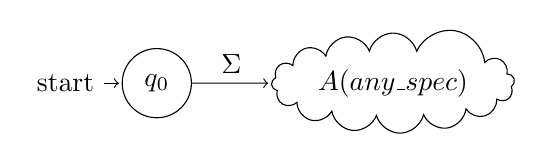
\begin{tikzpicture}[shorten >=1pt,node distance=3cm,on grid,auto,scale=.5]
			\node[state,initial] (q0)									{$q_0$};
			\node[cloud, cloud puffs=15.7, cloud ignores aspect, align=center, draw] (q1) [right of=q0]
			{$A(any\_spec)$};
			\path[->]
				(q0) edge node {$\Sigma$} (q1);
		\end{tikzpicture}
		\subcaption{The \textit{next specification}, as an automaton.}
	\end{minipage}

	\caption{The \textit{next specification} - the specification that deals with
	time.}
	\label{label-spec-next}
\end{figure}

%%%%
%% if spec
\begin{figure}[h!]

	\begin{minipage}{0.45\textwidth}
		\centering
		\lstset{language=Python}
		\begin{lstlisting}
		def if_spec():
			if P0:
				innerspec_0() # next or null spec
			# optional additional conditionals, 1 to n-1
			else if Pi:
				innerspec_i() # next or null spec
			# optional else clause
			else:
				innerspec_n() # next or null spec

		\end{lstlisting}
		\centering
		\subcaption{The \textit{if specification}, in python function format.}
	\end{minipage}



	\begin{minipage}{0.45\textwidth}
		\centering
		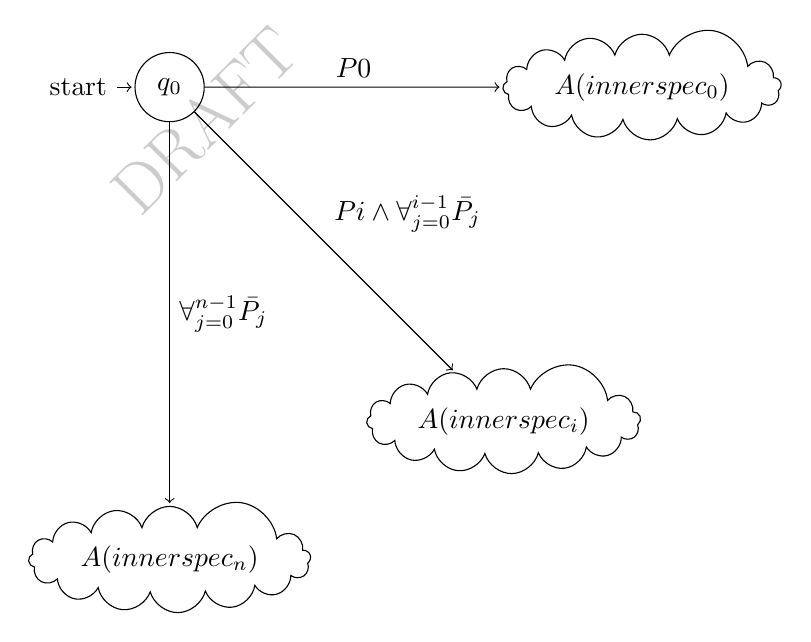
\begin{tikzpicture}[shorten >=1pt,node distance=6cm,on grid,auto,scale=.5]
			\node[state,initial] (q0)									{$q_0$};
			\node[cloud, cloud puffs=15.7, cloud ignores aspect, align=center, draw] (q1) [right of=q0] {$A(innerspec_0)$};
			\node[cloud, cloud puffs=15.7, cloud ignores aspect, align=center, draw] (q2) [below right of=q0] {$A(innerspec_i)$};
			\node[cloud, cloud puffs=15.7, cloud ignores aspect, align=center, draw] (q3) [below of=q0] {$A(innerspec_n)$};
			\path[->]
				(q0) edge node {$P0$} (q1)
				(q0) edge node {$Pi \wedge \forall_{j=0}^{i-1} \bar{P_j}$} (q2)
				(q0) edge node {$\forall_{j=0}^{n-1} \bar{P_j}$} (q3);
		\end{tikzpicture}
		\centering
		\subcaption{The \textit{if specification}, as an automaton.}
	\end{minipage}

	\caption{The \textit{if specification} - the most complex specification.}
	\label{label-spec-if}
\end{figure}




%================================================
%====== Chapter 5, Results
%================================================

\pagestyle{newchap}
\chapter{Results} \label{chapter-results}

Mm.




%================================================
%====== Chapter 6, Conclusions
%================================================

\pagestyle{newchap}
\chapter{Conclusions}
Yay, it worked!


\section{Discussion}

What do we see in the future? How can this be extended, continued?

Results (un)expected? Larger context.

Some speculation? Recommendations?

\section{Future Work}


Some temporary citations:
\cite{hoare69}, \cite{floyd67}, \cite{pnueli77}, \cite{leucker09abriefaccount},
\cite{bauer06monitoring}, \cite{bauer08goodbadugly}, \cite{delgado04taxonomy},
\cite{meyer92applyingdbc}, \cite{rosenblum95practicalassertions},
\cite{bartetzko01jass}, \cite{bodden04lightweightltl},
\cite{bodden05efficientrv}, \cite{becksmalltalktesting}, \cite{fowlerxunit},
\cite{matusiak09aoppy}




%================================================
%====== Bibliography
%================================================

% the ieeetr style orders the references after first appearance
\bibliographystyle{ieeetr}
\bibliography{references}




%================================================
%====== Appendices
%================================================

% no appendices yet

\end{document}
